\documentclass[10pt]{article}

% amsmath package, useful for mathematical formulas
\usepackage{amsmath}
% amssymb package, useful for mathematical symbols
\usepackage{amssymb}

% graphicx package, useful for including eps and pdf graphics
% include graphics with the command \includegraphics
\usepackage{graphicx}
\usepackage{epstopdf}
\graphicspath{ {./figures/} }

% cite package, to clean up citations in the main text. Do not remove.
\usepackage{cite}
\usepackage{color}
\usepackage{soul}
\usepackage{longtable}
\usepackage{pdfpages}
\usepackage{color}

% Text layout
\topmargin 0.0cm
\oddsidemargin 0.5cm
\evensidemargin 0.5cm
\textwidth 16cm 
\textheight 21cm

% Bold the 'Figure #' in the caption and separate it with a period
% Captions will be left justified
\usepackage[labelfont=bf,labelsep=period,justification=raggedright]{caption}


\bibliographystyle{plain}

% Remove brackets from numbering in List of References
\makeatletter
\renewcommand{\@biblabel}[1]{\quad#1.}
\makeatother


% Leave date blank
\date{}

\pagestyle{myheadings}
%% ** EDIT HERE **

\newcommand{\beginsupplement}{%
        \setcounter{table}{0}
        \renewcommand{\thetable}{S\arabic{table}}%
        \setcounter{figure}{0}
        \renewcommand{\thefigure}{S\arabic{figure}}%
     }


%% END MACROS SECTION

\begin{document}

% Title must be 150 characters or less
\begin{flushleft}
{\Large
\textbf{The Metabolic Landscape of Tumors}
}
% Insert Author names, affiliations and corresponding author email.
\\
E Reznik, A Luna, BA Aksoy, C Sander, others less worthy
\\
$^1$ Computational Biology Center, Sloan-Kettering Institute, New York NY

$^\ast$ E-mail: reznike@mskcc.org
\end{flushleft}

\begin{abstract}
\end{abstract}

\section{Introduction}

The metabolism of tumors and normal tissue is aligned toward the same objective: to derive energy and cellular building blocks from the environment. Furthermore, both cancers and normal cells are endowed with an identical repertoire of metabolic enzymes and nutrient transporters, encoded in the human genome. Thus, to 


\begin{figure}[ht!]
  \centering
     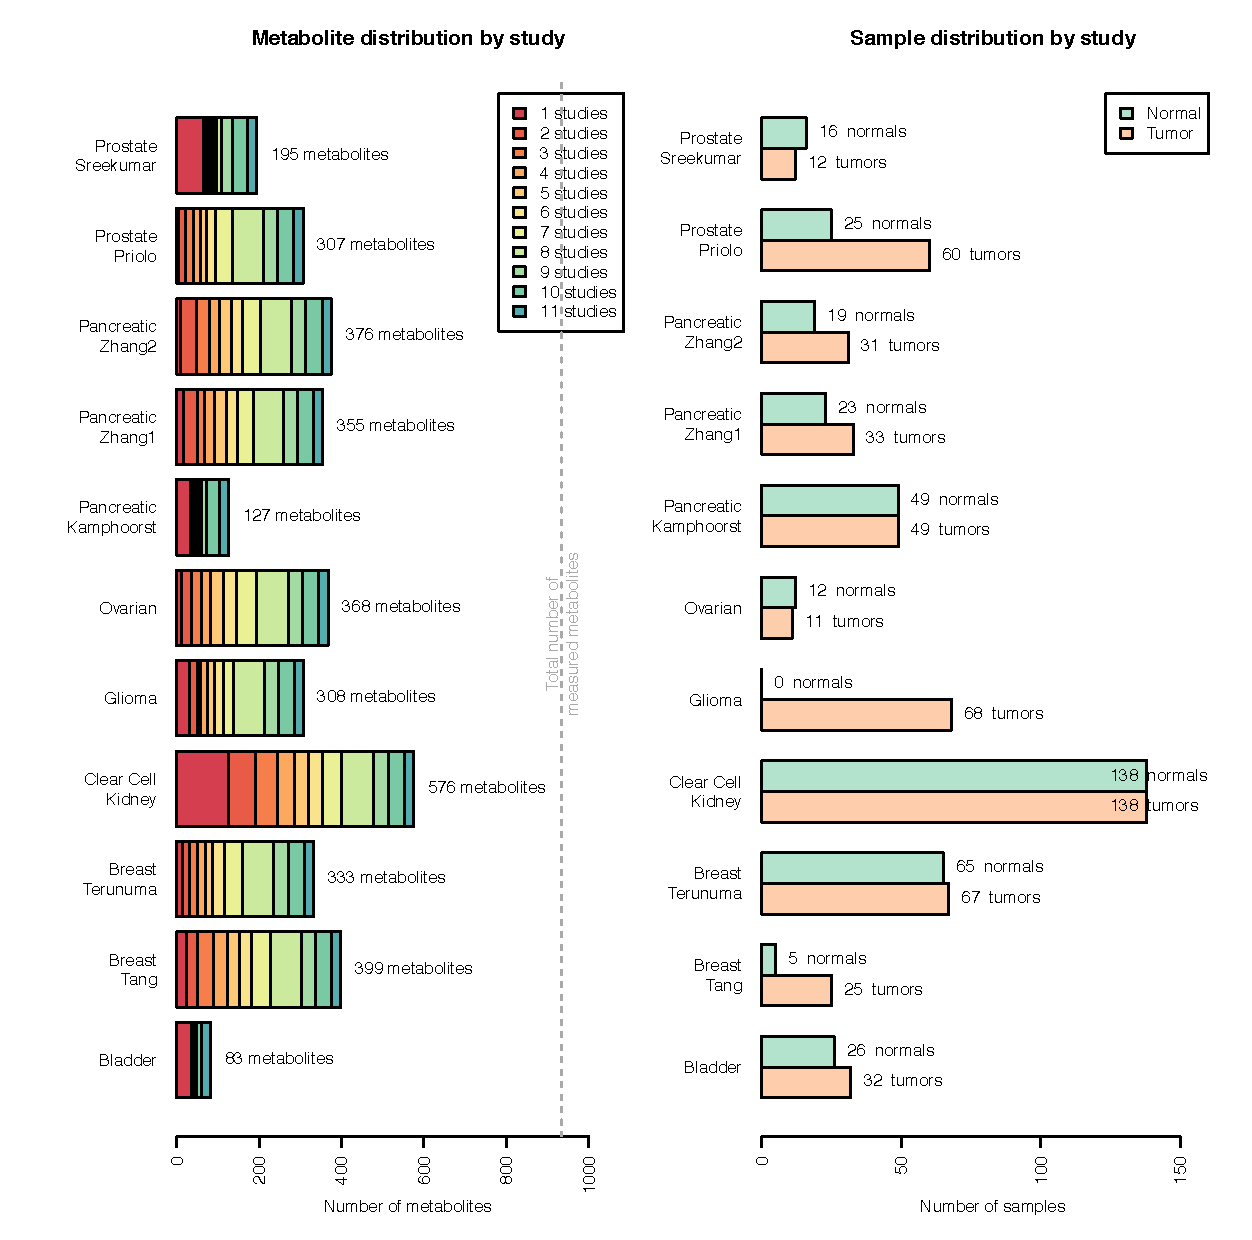
\includegraphics[scale = 0.5]{figures/Figure1/Figure1.pdf}
  \caption{Insert caption. }
     \label{fig:Fig1}
\end{figure}

\section{Assembly of a Cross-Cancer Compendium of Metabolomics Data}
We obtained published cancer tissue metabolomics data from twelve studies examining nine distinct cancer types. The goal of our study was to assemble the data from these studies into a coherent, unified dataset in which measurements of metabolites could be compared across studies. The compilation of metabolomic data was difficult for two readsons, broadly falling into the categories of data standardization and bioinformatic messiness.

A major challenge in integrating metabolomics data from multiple studies is data standardization. Data generated from mass spectrometry studies was reported as peak intensity values, which are not an absolute measure of concentration (unless there is a spiked-in reference). Therefore, data from these studies is reported as a relative quantification of a metabolite, relative to the median abundance of that metabolite across all samples in the study. As a consequence, the abundance of a metabolite $i$ in sample $j$ could only be directly compared to measurements of metabolite $i$ in other samples in the same study, but not to measurements of  (1) other metabolites in the same study, or (2) metabolite $i$ in other studies. Furthermore, due to metabolite abundances which fell outside the sensitivity of the measuring instrument, a substantial number of measurements were either missing or imputed. As depicted in Figure 1, we implemented a simple and consistent methodology for standardizing metabolite abundances for each study. 

The second major challenge was correctly identifying metabolites commonly sampled across many studies. In contrast to genes, which have a commonly accepted nomenclature, metabolites are ambiguously referred to by several names (\textit{e.g.} citrate, citric acid), and may be reported alongside an arbitrary subset of reference identifiers (\textit{e.g.} KEGG, Chebi, Pubchem, HMDB). To overcome this problem, we developed an automated pipeline to query a curated database of metabolite synonyms, based on a seed (typically, a single identifier). Then, a semi-automated script uses the expanded list of identifiers to assemble a unified metabolomic dataset (SI Data XX). Further details of the assembly process can be found in the Methods.

\begin{figure}[ht!]
  \centering
     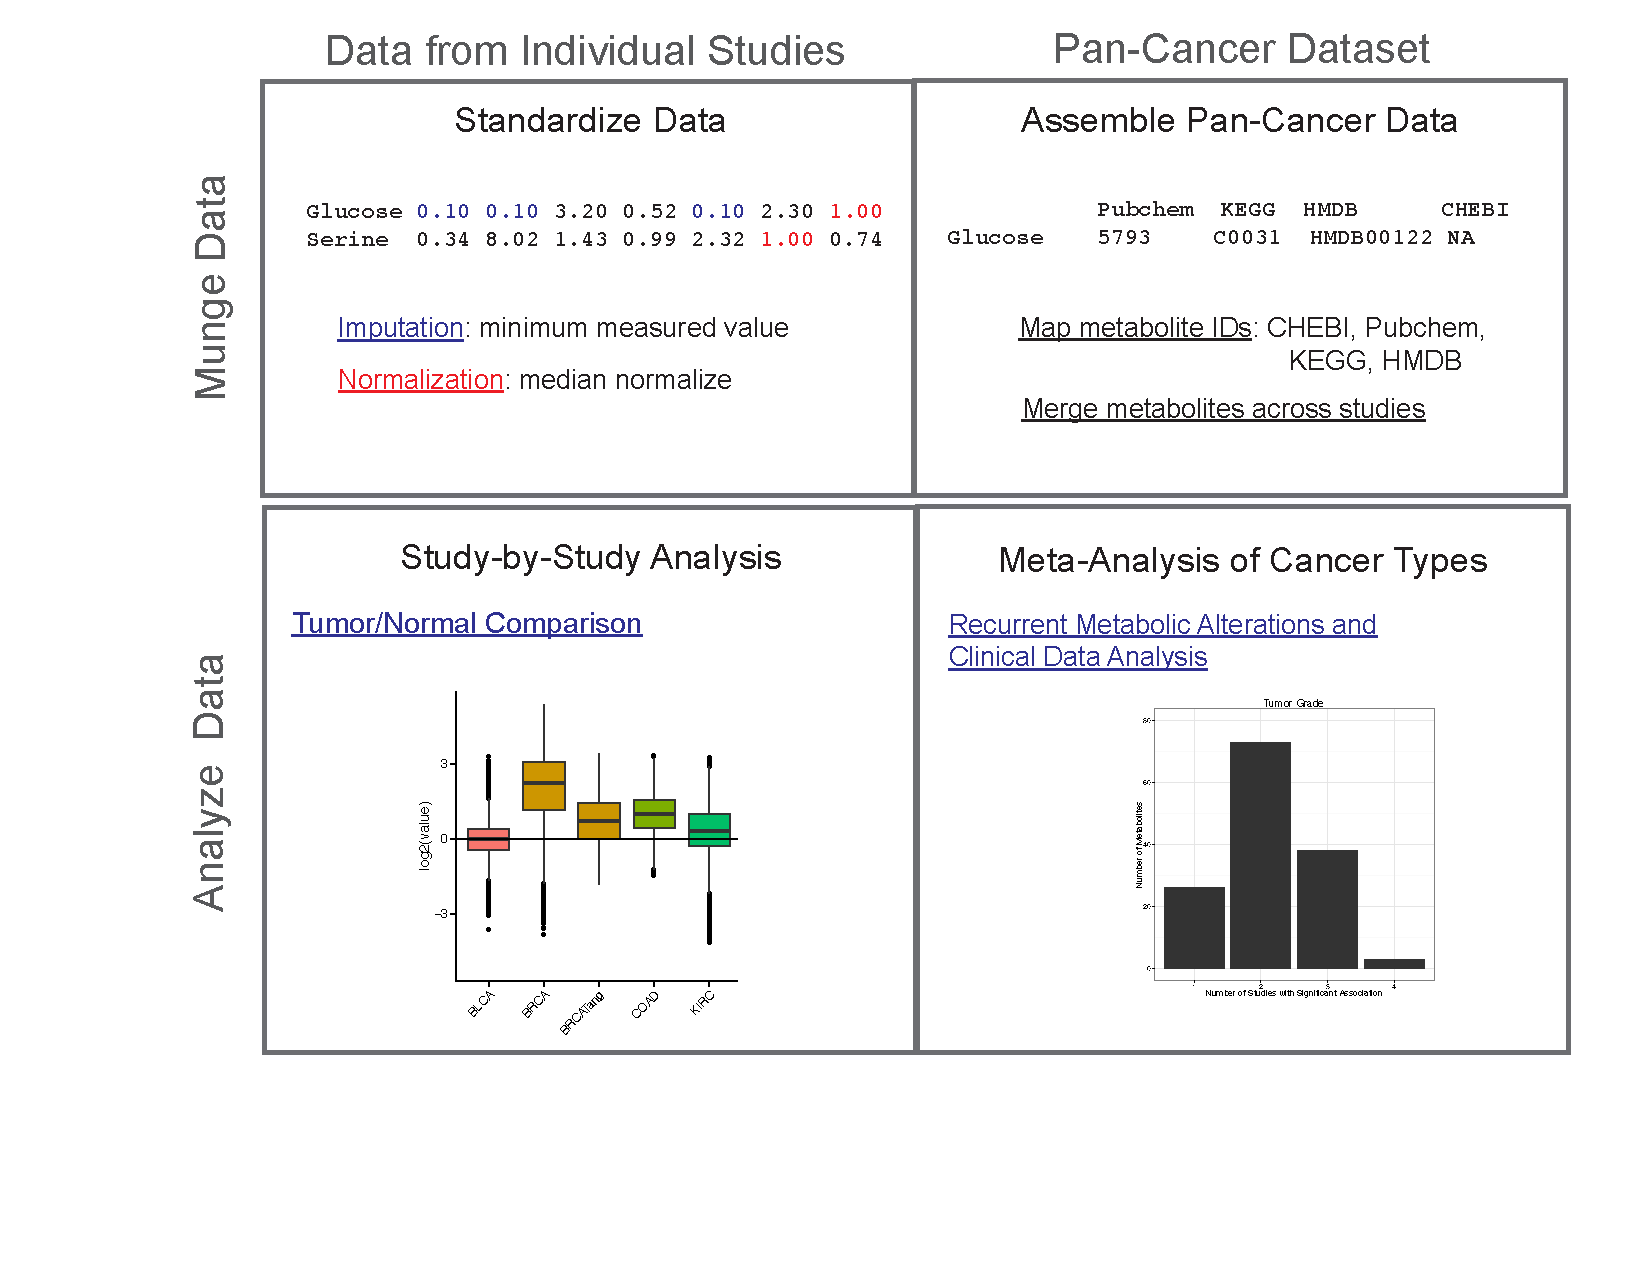
\includegraphics[scale = 0.5]{figures/Figure2/Figure2_workflow.pdf}
  \caption{Insert caption. }
     \label{fig:Fig2}
\end{figure}

\textbf{Write here about cancer metabolomics data explorer}

\subsection{Tumors Are Not Necessarily Different From Normal Tissue?}

We began with a relatively simple question: how similar are tumors to their normal tissue counterparts? In other words, are the metabolic changes associated with transformation to cancer greater than the natural metabolic variation one might observe in normal tissue? To estimate similarity, we calculated a metabolic distance between each pair of tissue samples in a study (see Methods). We then examined how the typical distance between a tumor and normal sample compared to the analagous distance between two normal samples, for a given cancer type. We found that some cancer types (including clear-cell kidney and breast cancers) were highly dissimilar from their normal tissue counterparts. At the other end of the spectrum, we also found that prostate and pancreatic tumors displayed a surprisingly small amount of variation, compared to the variation of normal prostate and pancreatic tissue, respectively. Importantly, this effect was evident in both prostate cancer studies in our meta-dataset, as well as all three pancreatic cancer studies.

An orthogonal method for analyzing high-dimensional data, and one that is conventionally used as a first-step during analysis, is to project it onto a highly informative, low-dimensional space using performed principal components analysis (PCA).  Upon applying PCA to each dataset in our meta-analysis, we found that the majority of cancer types displayed a clear separation of tumor and normal samples. Surprisingly, however, we again found that prostate tumors and pancreatic tumors displayed poor to no separation from their respective normal samples using the first 2 principal components (see SI Figs XX-XX, evident in both prostate studies and all three of the pancreatic studies). Together with the results in Figure XX, these observations suggest that prostate and pancreatic tumors exhibit relatively small changes in the process of transformation, when compared to the natural metabolic variation evident in normal tissues.

\section{Detailed Examination of Metabolic Alterations Across Cancer Types}
The perplexing observation that prostate and pancreatic tumors showed relatively minor changes in metabolite abundances compared to normal tissue led us to investigate the phenomenon in more detail. To do so, we examined, on a study-by-study basis, which metabolites were differentially abundant between tumor and normal samples. We found the number of differentially abundant metabolites varied drastically from one cancer type to the next (Figure XX). For example, in studies of breast and clear-cell kidney tumors, we found that greater than 40 percent of metabolites showed at least a 2-fold change in abundance, whereas two independent studies of prostate cancer found that fewer than 6 percent of metabolites were differentially abundant. Importantly, because the number of tumor/normal samples were comparable for these two cancer types, the differences in differential abundance were unlikely to be statistical artifacts arising from differences in sample size \textcolor{red}{(should we include additional analysis, ie boostrapping?)}.

This analysis also revealed a cancer-type-dependent trend towards unequal proportions of metabolites which increased or decreased between tumor and normal tissues. In both breast cancer studies, we found that nearly all metabolites deemed differentially abundant were at higher levels in tumor tissue, compared to normal tissue. While similar biases were evident in other studies (\textit{.e.g.} differentially abundant metabolites in pancreatic tumors tended to be at lower concentration in tumors), the effect was particularly striking for breast cancers. Although it is not possible for us to determine with certainty the source of this effect, we speculate it could arise from the imbalance between imputation in tumors and normal tissue. In particular, both breast cancer studies were exceptional for containing substantially more metabolites which were imputed in normal tissues, compared to tumor tissues.

\begin{figure}[ht!]
  \centering
     \includegraphics[scale = 0.5]{figures/Figure3/Figure3.pdf}
  \caption{Insert caption. }
     \label{fig:Fig3}
\end{figure}

\section{ Common Patterns of Metabolic Alterations Across Cancers}
A key question or us was whether a subset of metabolites showed consistent patterns of increased/decreased abundance in tumors, relative to adjacent-normal tissues. The existence of such metabolites could be indicative of a cross-cancer signature of transformation. By aggregating the results of our differential abundance screen, we identified 113 metabolites differentially abundant in at least 5 studies. Among these, a single metabolite, taurine, was differentially abundannt in ten of the twelve studies in which it was measured. Two TCA cycle metabolites (fumarate and malate), and a number of amino acids, including aspartate, asparagine, arginine, methionine, and proline, were differentially abundant in 8 studies. In all cases, the direction of change (\textit{i.e.} higher or lower in tumor, relative to normal) was not consistent across cancer types.

To identify metabolic alterations characteristic of transformation, we focused on metabolites which showed recurrent, consistent changes in abundance across tumor types. Two metabolites, lactate and kynurenine, were observed to increase in abundance in 8 tumor types (and decrease in abundance in zero). The fate of pyruvate, the terminal product of glycolysis, is binary: it can be converted to acetyl-CoA and oxidized in the TCA cycle, or to lactate for excretion. A wealth of literature has suggested that, for a number of reasons (as discussed in XXX), tumors increase their production of lactate, a finding which is recapitulated in this study. In the ensuing sections, we will examine in more detail the characteristics of tumors which do/do not display increased levels of lactate and kynurenine. 

We also identified three metabolites which showed recurrent down-regulation in tumors: caprate, pelargonate, and guanidoacetic acid, which each showed downregulation in 4 distinct studies (\textcolor{red}{which studies?}). Both caprate and pelargonate are medium chain fatty acids, with chain lengths of ten and nine, respectively, while guanidoacetate is an intermediary metabolite of the TCA cycle. Interestingly, laurate, a medium chain fatty acid of carbon chain length 12, also showed a tendency towards recurrent downregulation (decreased in abundance in tumors in 4 studies, increased in abundance in one). 

Finally, we aggregated our differential abundance analysis results in order to conduct pathway analysis. For each study, we mapped metabolites onto the KEGG pathways they were members of, and calculated an aggregate differential abundance score for each pathway. We observed a tendency across cancers for increases in central carbon metabolism (including the pathways glycolysis/gluconeogenesis, fructose and mannose metabolism, and propanoate metaoblism), and a general down-regulation of lipid and fatty acid pathways (such as glycerolipid metabolism and fatty acid biosynthesis). Interestingly, we observed that while metabolites in the TCA cycle and oxidative phosphorylation were frequently differentially abundant, their direction of change (\textit{i.e.} higher or lower in tumors) varied across cancer types, echoing a similar finding in a pan-cancer analysis of metabolic gene expression data.

\begin{figure}[ht!]
  \centering
     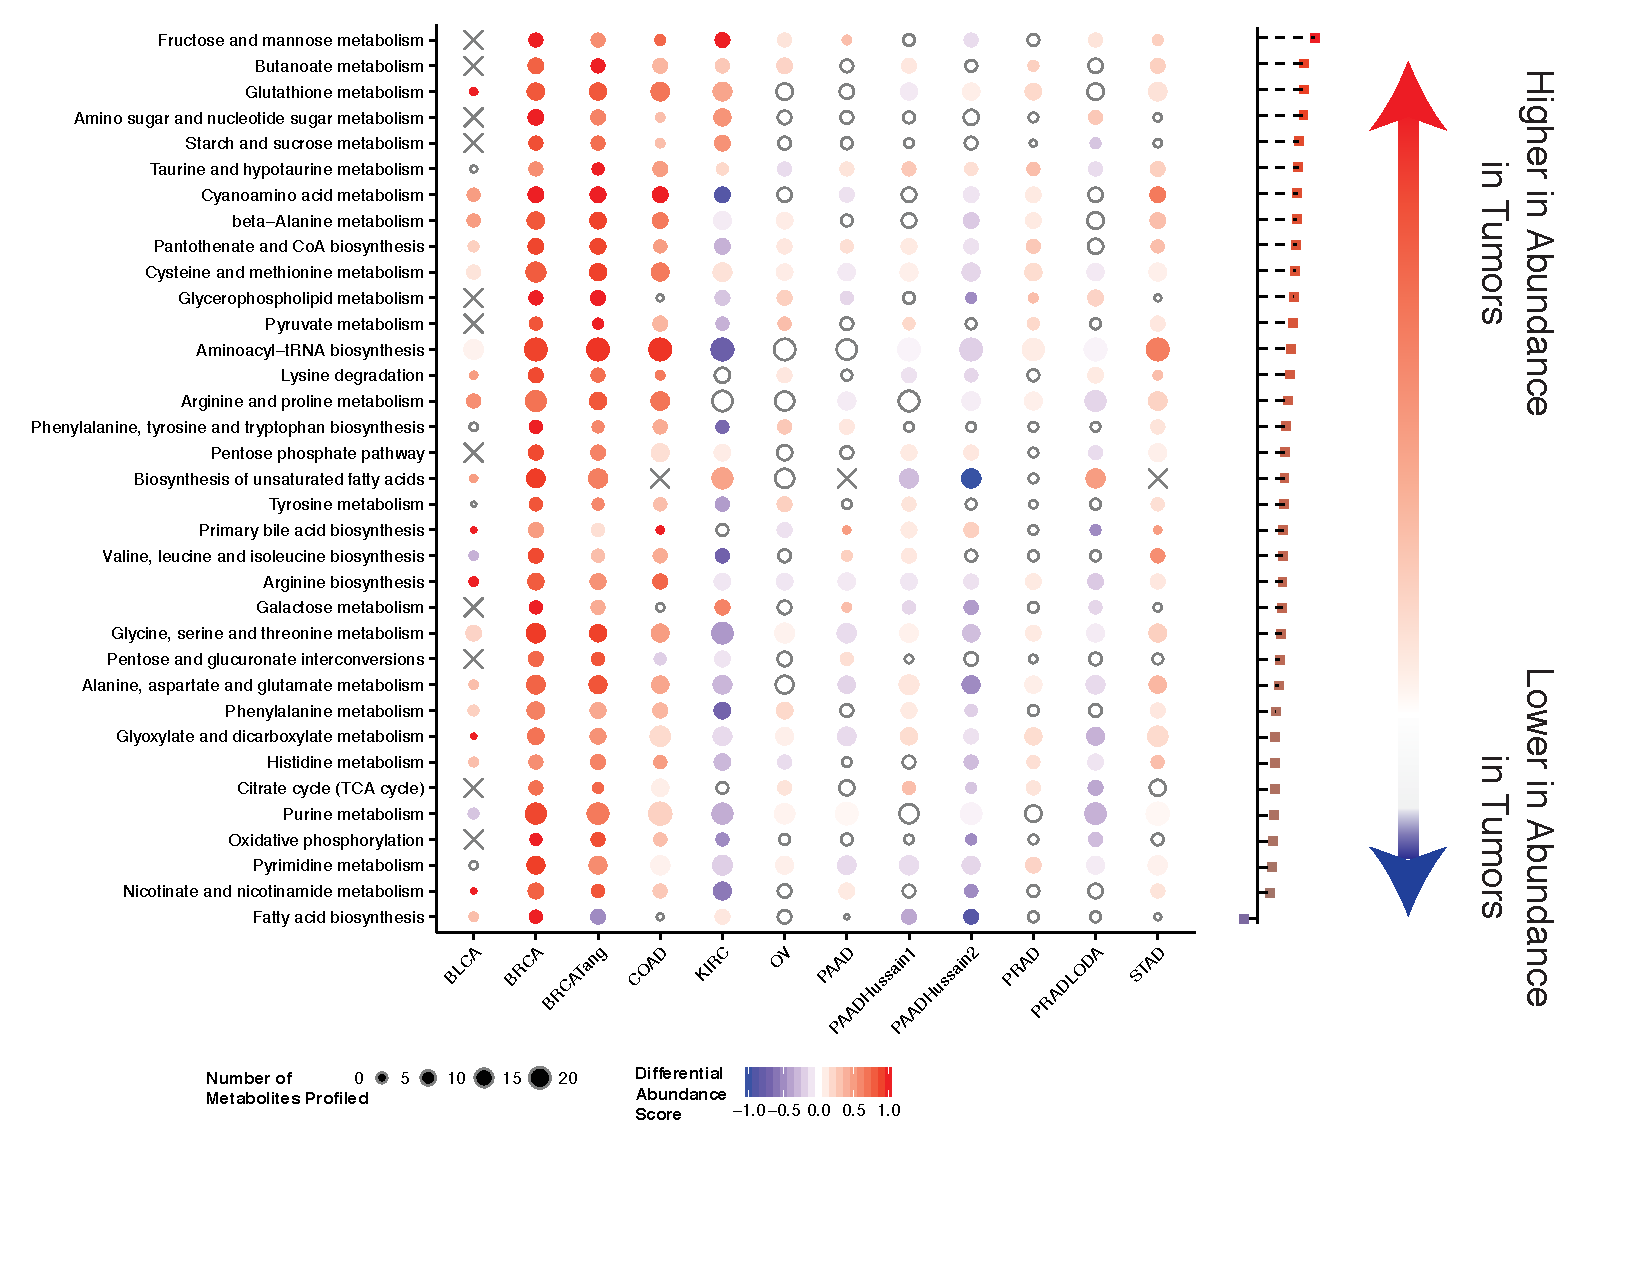
\includegraphics[scale = 0.5]{figures/Figure4/Figure4.pdf}
  \caption{Insert caption. }
     \label{fig:Fig4}
\end{figure}


\section{Metabolic Correlations with Tumor Progression}
A key question for our analysis was understanding whether certain metabolties were associated with the progression of tumors to higher grade and more aggresive stage. The studies that we collected frequently reported at least one of two measures of cancer progression: tumor grade and tumor stage. Tumor grade is a histological measure of the extent of abnormal apperance of tumor cells. In contrast, tumor stage describes the severity of a tumor based on its size, infilitration of lymph nodes, and metastatic status. Among the 12 cancer studies which we collected in our dataset, XX had associated clinical data on tumor stage or grade. We used statistical meta-analysis techniques to identify metabolites which showed consistent changes (\textit{i.e.} consistent increase/decrease in metabolite levels with increasing tumor stage) across several cancer types. Our analyis accounted for the frequency of imputed data (see detailed description in Methods).

In total, we found 140 metabolites whose abundance were significantly correlated to tumor grade, and 60 metabolites with abundances significantly correlated to tumor stage. Filtering these results further to extract metabolites significantly associated with clinical features across many tumor types, we found 2 metabolites, erythronate and cytidine 5'-diphosphocholine, significantly associated to tumor stage in breast kidney, and ovarian cancers. We found 14 metabolites associated to tumor grade in at least 3 studies, including several amino acids (asparagine, proline, phenylalanine, leucine), 3 pyrimidines and their derivatives (thymine, uracil, and 5,6-dihydrouracil), and kynurenine. 

Among the most interesting findings was the observation that kynurenine levels were increased in tumors versus normal tissues. Kynurenine is a metabolic byproduct of the degradation of trytophan by two groups of enzymes: tryptophan dioxygenases and indoleamine 2,3-dixoygenases. Binding of kynurenine to aryl hydrocarbon receptors (AHRs) and suppress the activity of T-effector cells, as well as indirectly activating regulatory pro-tumorigenic T cells. Kynurenine was unique in our study because it was found to be elevated in the majority of tissues, and it was also found to be positively correlated to tumor grade in 4 different studies (2 different prostate cancer studies, as well as breast cancers and gliomas). Together, these findings point to a critical role for kynurenine in the metabolism of tumors.

\begin{figure}[ht!]
  \centering
     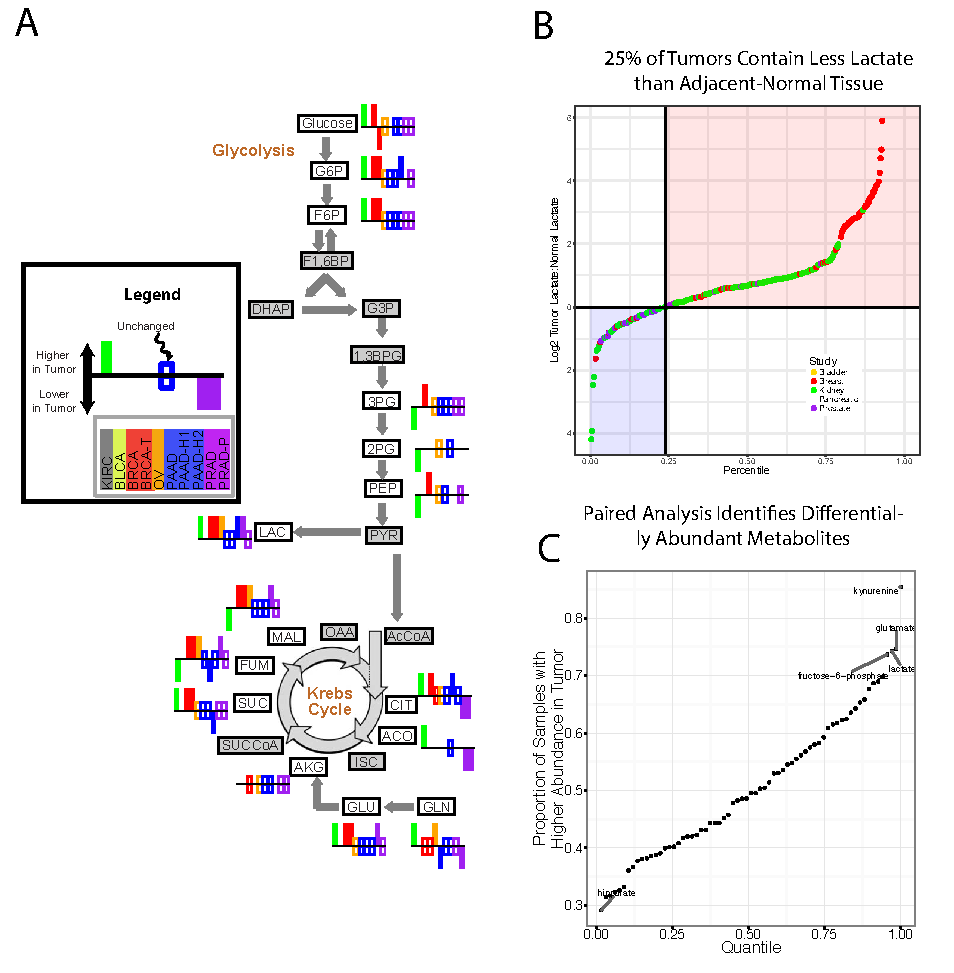
\includegraphics[scale = 0.5]{figures/Figure5/Figure5.pdf}
  \caption{Insert caption. }
     \label{fig:Fig5}
\end{figure}

\section{Incidence of the Warburg Effect Across Cancers }
The canonical observation of Otto Warburg, during his seminal studies of cancer metabolism in 19XX, was an increase in the concentration of lactate in tumor tissues. Since then, the so-called ``Warburg effect'' has been studied extensively across many systems, and has been attributed to shift away from aerobic metabolism in tumors. However, it is also well-established that mitochondrial metabolism, including both oxidative phosphorylation and other metabolic activities, is crucial to the proliferation of tumors.

We examined whether levels of lactate, a metabolic end-product of aerobic glycolysis and a commonly used surrogate for the extent of the Warburg effect in a tumor sample, were elevated in tumors compared to matched normal tissues. Surprisingly, we observed that nearly a quarter of all tumor samples were depleted of lactate, relative to their matched, adjacent-normal tissue. Excluding colorectal adenocarcinomas, each tumor type with available adjacent-normal tissue contained at least one paired tumor/normal sample exhibiting a depletion of lactate. The effect was particularly pronounced among prostate cancers. In both studies examining prostate cancers, the majority of tumors were actually depleted of lactate.

Our use of adjacent-normal tissue as a standard by which to examine changes in lactate levels is not entirely fair: it is possible that, for a given sample, the level of lactate in the normal tissue may be exceptionally high. We examined whether the apparent depletion of lactate was further due to 

\begin{figure}[ht!]
  \centering
     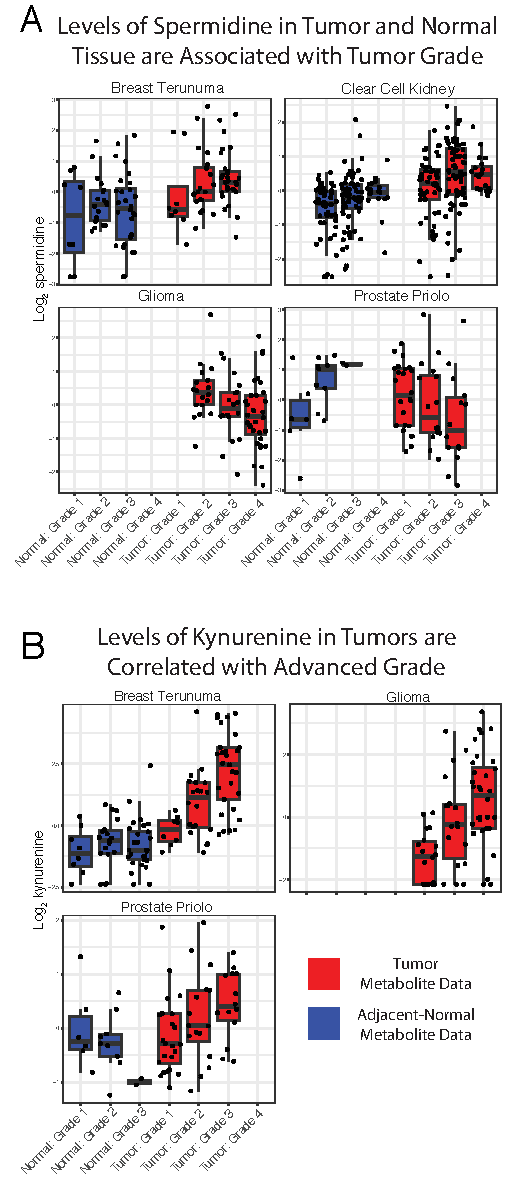
\includegraphics[scale = 0.5]{figures/Figure6/Figure6.pdf}
  \caption{Insert caption. }
     \label{fig:Fig6}
\end{figure}

\section{Discussion}

\subsection{Data Integration}
The majority of the data we collected was derived from measurements of metabolites on a relative scale. In other words, the  abundance of a metabolite was relative to other measurements of the same metabolite in the same study (\textit{i.e.} a measurement of glucose in one study could not be directly compared to a measurement of glucose in another). Furthermore, because most of the data in our analysis was derived from mass spectrometry, a substantial fraction of measurements were reported to fall below the detection threshold of the instrument. Such data is frequently reported as ``NA'' in the corresponding published data. Making this data amenable to quantitative analysis was essential for us, because it contained useful information indicating that the concentration of a metabolite was low (compared to samples where the concentration was within the quantifiable limits). Therefore, we followed prior work and applied an imputation procedure to enable use of these measurements in our analysis.We proposed a straightforward approach, based on fold change relative to matched normal tissue, to enable comparison across cancer types. 

Perhaps the first challenge we encountered during data collection was the difficulty of ``aligning'' a metabolite which had been profiled in more than one study, but was labeled with a distinct name (\textit{e.g.} lactate, lactic acid, L-lactate, (S)-lactate)). Typically, metadata regarding the chemical identity of metabolites (\textit{i.e.} KEGG IDs, PubChem IDs) was included in studies, but this metadata was universally incomplete. In most cases, a study would include either a KEGG ID or an HMDB ID for a metabolite, but not both. This made the task of finding common metabolites across studies exceptionally challenging. To overcome this challenge, we developed a bioinformatic method for assembling a list of consistent metabolite identifiers for each metabolite profiled in each study.

A second challenge arose from the large amount of incomplete data. 

Third, nearly all of the data in the meta-analysis (with the exception of the COAD/STAD data) 

The final, and perhaps most challenging, complication of our data was that, because of incomplete coverage of the metabolome, very few metabolites were profiled across more than a small number of studies. This challenge became increasingly important to address when attempting to cluster the metabolomics data across many tumor types, because the number of metabolites concordantly sampled varied from one pair of studies to the next. As a result, the dimensionality of the data varied from one pair of samples to the next, making calculating distances challenging. We proposed a non-parametric clustering approach which handled incongruous dimensionality, and showed that it identified an outlying cluster of ccRCC tumors distinguished by elevated levels of dipeptides.


\subsection{Cross-Cancer Comparison of Metabolomics Data}


\section{Methods}

\subsection{Differential Abundance Tests}
Differential abundance was calculated using the ratio of the average abundance of a metabolite in tumor tissue, to the average abundance of a metabolite in normal tissue. Statistical significance was assessed using non-paramatric Mann-Whitney U-tests.

\subsection{Pathway Differential Abundance Score}
The differential abundance score for a pathway was defined as

\begin{align*}
DA = \frac{I - D}{S}
\end{align*}

\noindent where $I$ is the number of measured metabolites in a pathway which increased in abundance relative to normal tissue, $D$ is the number which decreased, and $S$ is the total number of measured metabolites. A $DA$ score of 1 indicates that all metabolites increased in abundance, whereas a score of -1 indicates that all metabolites decreased in abundance, relative to normal tissue.

\subsection{Metabolomics Data Acquisition and Normalization}
Metabolomics data from prior, published work was obtained either through the corresponding journal, or by contacting the corresponding author. The data for all studies except COAD and STAD was reported in relative abundances, \textit{i.e.} the abundance of a metabolite $i$ in sample $j$ could only be compared to other values of metabolite $i$ in different samples from the same study. For COAD and STAD, absolute abundances were reported.

Because metabolomics data does not necessarily obey a known distribution, we applied minimal normalization techniques in order to make data minimally comparable across all studies. For each metabolite in a study, we calculated the median abundance, and normalized by this abundance. Given the unknown distribution of the data in our study, we used only non-parametric statistical tests (which are independent of data distribution) to assess changes in metabolite abundance.

\subsection{Association with Stage and Grade}
Different statistical tests were applied to identify correlation between metabolites and clinical features depending on the level of censoring in the data. If there is less than 20\% censoring within the tested set, the Jonckheere-Terpstra test (a non-parametric test which uses permutations to calculate the p-value) was used to examine ordered differences among classes . If there are more than 20\% but less than 80\% censored data, an exact log-rank trend test is used for interval (left) censored data. Both tests assume a metabolite should increase/decrease monotonically with stage/grade.  If there is more than 80\% censoring no test is used, and the metabolite is ignored. To summarize the tests across cohorts I use Fisher’s method to combine p-values. Note that resulting combined p-value is parametric. 

Since we are interested in finding associations of a common sign (\textit{e.g.} consistently positive correlation across multiple studies), one-sided p-values are calculated first, aggregate into a combined p-value using Fisher's method (CITE), and then transformed to two-sided combined p-value.

\beginsupplement

\begin{figure}[ht!]
  \centering
     \includegraphics[scale = .6]{figures/SIFigures/imput_barplot.pdf}
  \caption{Insert caption.}
     \label{fig:SIFig_Imputation}
\end{figure}

\begin{figure}[ht!]
  \centering
     \includegraphics[scale = .6]{figures/SIFigures/sametissue.pdf}
  \caption{Insert caption.}
     \label{fig:SIFig_SameTissue}
\end{figure}

\begin{figure}[ht!]
  \centering
     \includegraphics[scale = .6]{figures/SIFigures/Histogram_NumDiffAbundant.pdf}
  \caption{Insert caption.}
     \label{fig:SIFig_HistogramDiffAbundance}
\end{figure}
 

\begin{figure}[ht!]
  \centering
     \includegraphics[scale = .6]{figures/SIFigures/pathway_heatmap.pdf}
  \caption{Insert caption.}
     \label{fig:SIFig_PathwayHeatmap}
\end{figure}

\begin{figure}[ht!]
  \centering
     \includegraphics[scale = .6]{figures/SIFigures/warburg_source.pdf}
  \caption{Insert caption.}
     \label{fig:SIFig_WarburgSource}
\end{figure}
 
\end{document}
